\documentclass[11pt,leqno]{article}
\usepackage{amsmath}
\usepackage{amsthm}
\usepackage{amstext}
\usepackage{amsopn}
\usepackage{texdraw}
\usepackage{graphicx}
\usepackage{color}
\oddsidemargin 0in \topmargin 0in \textwidth 6.2in \textheight 8.2in
\baselineskip=20pt
\parskip=2mm
\parindent=20pt

\DeclareMathOperator{\codim}{codim}
\DeclareMathOperator{\Span}{span}
\newtheorem{theorem}{Theorem}[section]
\newtheorem{lemma}[theorem]{Lemma}
\newtheorem{proposition}[theorem]{Proposition}
\newtheorem{corollary}[theorem]{Corollary}

\theoremstyle{definition}
\newtheorem{definition}[theorem]{Definition}
\newtheorem{example}[theorem]{Example}
\newtheorem{xca}[theorem]{Exercise}

\theoremstyle{remark}
\newtheorem{remark}[theorem]{Remark}

\numberwithin{equation}{section}



\begin{document}
\title{Inverse Problem and Super Central Configurations of the Collinear $5$-body Problem }
\author{Davis, Geyer, Johnson, Xie  \\
Department of Mathematics\\
The University of Southern Mississippi\\
Hattiesburg, Mississippi 39406, USA\\
 Email: zhifu.xie@usm.edu }
\date{}

\maketitle
\begin{abstract}
 In this paper we study the inverse problem of collinear central configurations: given a collinear configuration $x$ of $n$ bodies, find the set of masses $S(x)$ which make it central. %The determination of the set of masses $S(x)$ depends on an associated Pfaffian. We provide a simple analytical proof of that the associated Pfaffian is nonzero for any given noncollision configuration in the collinear $n$ body problem with $n\leq 6$. Therefore the set of masses $S(x)$ is two-dimensional. A configuration $x=(x_1, x_2, \cdots, x_n)$ is called a supercentral configuration if there exists a positive mass vector$m=(m_1,\cdots, m_n)$ such that  $m\in S(x)$ and $m^\prime\in S(x)$ where $m^\prime$  is a permutation of $ m $ and $m^\prime \not=m $. Let $S_m(x)$ be the set of permutations $m^\prime$ of $m$ such that $m^\prime\in S(x)$. For any noncollision configuration $x$ in the collinear $n$-body problem with $n\leq 6$ and any $m\in S(x)$, either $^\#S_m(x)=0$ or $^\#S_m(x)=1$. The results could be extended for general noncollision collinear configuration of $n$ bodies provided that the associated Pfaffians are nonzero.  %This paper partially answered the questions raised by Moulton in his paper [The Annals of Mathematics,Vol 12. No. 1 (1910). pp. 1--17].
\end{abstract}

{\bf Key words:} Skew Symmetric Matrix, Determinant, Pfaffin, Central Configurations, Super Central Configurations. \\
{\bf AMS classification number:} 37N05, 70F10, 70F15,
37N30, 70H05.\\

\section{Introduction and Main Results}
\setcounter{section}{1} \setcounter{equation}{0}

We use the same notation as the paper \cite{ZX6}. A configuration $x=(x_1, x_2, \cdots, x_n)^T$ is called a central configuration for a mass vector  $m=(m_1, m_2, \cdots, m_n)^T$, if there exists $\lambda$ such that the following system of algebraic equations holds:
\begin{equation}\label{cc1}
 \left\{ \begin{array}{ll}
 0+\frac{m_2(x_2-x_1)}{r_{12}^3}+\frac{m_3(x_3-x_1)}{r_{13}^3}+\cdots+\frac{m_n(x_n-x_1)}{r_{1n}^3} &= -\lambda(x_1-c),\\
 %\\
  -\frac{m_1(x_1-x_2)}{r_{12}^3}+0+\frac{m_3(x_3-x_2)}{r_{23}^3}+\cdots+\frac{m_n(x_n-x_2)}{r_{2n}^3} &= -\lambda(x_2-c),\\
%\\
  -\frac{m_1(x_1-x_3)}{r_{13}^3}-\frac{m_2(x_2-x_3)}{r_{23}^3}+0+\cdots+\frac{m_n(x_n-x_3)}{r_{3n}^3} &= -\lambda(x_3-c)\\
  %\\
  \vdots  & \vdots\\
  %\\
   -\frac{m_1(x_1-x_n)}{r_{1n}^3}-\frac{m_2(x_2-x_n)}{r_{2n}^3}-\frac{m_3(x_3-x_n)}{r_{3n}^3} -\cdots-0 &= -\lambda(x_n-c).\\

   \end{array} \right.
\end{equation}
Here $m_i>0$ are the masses of the bodies, $x_i$ are their positions, $r_{ij}=|x_i-x_j|$, $c=\frac{\sum m_ix_i}{M}$ is the center of mass of the bodies and $M=\sum m_i$ is the total mass. 

There will be no loss of generality in selecting the notation so that the position vector $x=(x_1, x_2, \cdots, x_n)^T\in \mathbf{R}^n$ with $x_1<x_2<\cdots <x_n$ for the collinear $n$-body problem. With this choice of notation the system of equations \eqref{cc1} becomes
\begin{equation}\label{cc2}
Bm=-\lambda(x-cL),
\end{equation}
where $B=B(x_1,x_2,\cdots,x_n)=(a_{ij})$, $a_{ij}=\frac{1}{r_{ij}^2}$ and $a_{ji}=-a_{ij}$ if $i<j$ and $a_{ii}=0$, $L=(1,1,\cdots,1)^T$. $\lambda$ and $c$ are parameters. Matrix $B$ is called the associated matrix of the configuration $x$. % For short, the vector form that is a row vector or column vector is determinate by the context.

Matrix $B$ is skew-symmetric and its determinant can be written as a square of a polynomial in the matrix entries $a_{ij}$. This polynomial is called the Pfaffian $Pf(B)$ of the matrix $B$.  

We consider collinear $5$-body problem with the given configuration $x_1=-s-1$, $x_2=-1,$ $x_3=r,$ $x_4=1,$ $x_5=t+1$. Assume that $s, t\in (0, \infty)$ and $r\in (-1, 1)$.  The bodies are in the order of $x_1<x_2<x_3<x_4<x_5$. Let $a_{ij}=(x_j-x_i)^{-2}$  and $a_{ji}=-a_{ij}$ for $1\leq i<j\leq 5$.  $a_{ii}=0, i=1,2,\cdots, 5$. 

Let $A$ be the associate matrix of the configuration $\vec{b}=(x_1, x_2, x_4, x_5)^T$.
$$A=\left( \begin {array}{cccc} 0&  a_{12}& a_{14}& a_{15}
\\ \noalign{\medskip}-a_{12}&0& a_{24}& a_{25}
\\ \noalign{\medskip}-a_{14}&- a_{24}&0& a_{45}
\\ \noalign{\medskip}- a_{15}&- a_{25}&- a_{45}&0\end {array}
 \right).
$$
{\bf $A$ is invertible for any given configuration $\vec{b}$. more information }
$$Pf(A)=  a_{12}  a_{45}- a_{14} a_{25}+ a_{15} a_{24}.$$
$$A^{-1}= \frac{1}{Pf(A)}\left( \begin {array}{cccc} 0&-a_{45}& a_{25}&- a_{24}
\\ \noalign{\medskip}a_{45}&0&- a_{15}& a_{14}
\\ \noalign{\medskip}- a_{25}& a_{15}&0&- a_{12}
\\ \noalign{\medskip}a_{24}&- a_{14}& a_{12}&0\end {array}
 \right). 
$$
$$\vec{v}= \left( \begin {array}{cccc} - a_{13},&- a_{23},&a_{34},&  a_{35}
\end {array} \right)^T. $$
$$\vec{L}=\left( \begin {array}{cccc} 1,&1,&1,&1\end {array} \right)^T.$$
Then the four equations of collinear $5$-body central configuration equations involved $\vec{\tilde{m}}=(m_1, m_2, m_4, m_5)^T$ can be rewrote as 
$$A\vec{\tilde{m}}=-\lambda(\vec{b}-c\vec{L})+m_3\vec{v}.$$
Then
$$\vec{\tilde{m}}=-\lambda(A^{-1}\vec{b}-cA^{-1}\vec{L})+m_3A^{-1}\vec{v}.$$
Substitute it into the third equation and use the fact $\vec{v}^TA^{-1}\vec{v}=0$, we have
$$\vec{v}^{T}\vec{\tilde{m}}=-\lambda(x_3-c),$$
which is 
$$-\lambda(\vec{v}^{T}A^{-1}\vec{b}-c\vec{v}^TA^{-1}\vec{L})=-\lambda(x_3-c),$$
which implies 
$$c=\frac{x_3-\vec{v}^TA^{-1}\vec{b}}{1-\vec{v}^TA^{-1}\vec{L}}.$$

By using $m_1+m_2+m_3+m_4+m_5=M$, $m_3=M-\vec{L}^T \vec{\tilde{m}}=M+\lambda(\vec{L}^TA^{-1}\vec{b})-m_3\vec{L}^TA^{-1}\vec{v}$. So

$$m_3=\frac{\lambda \vec{L}^TA^{-1}\vec{b}+M}{1+\vec{L}^TA^{-1}\vec{v}}$$


\textcolor{red}{Prove: $c$ is well defined by showing the denominator is always bigger than 0.}\\
The following theorems have been proved in \cite{ZX6}. 
\begin{theorem}\label{thm5}
\begin{enumerate}
 \item The center of mass $c$ for any $5$-body collinear central configuration $x=(x_1,x_2,\cdots,x_5)^T$ only depends on the configuration $x$ and it is independent of the parameter $\lambda$ and the corresponding mass $m$. More precisely it is given by
\begin{equation}\label{cm}
c=\frac{x_3-\vec{v}^TA^{-1}\vec{b}}{1-\vec{v}^TA^{-1}\vec{L}},
\end{equation}
The denominator $1-\vec{v}^TA^{-1}\vec{L}$ of $c$ in \eqref{cm} is always positive for any configuration $x$.
\item With the appropriate choice of the center of mass $c$ given by \eqref{cm}, $m=(\vec{\tilde{m}}^T,m_3)^T$ can be given by a function with two parameters $\lambda$ and $m_3$
\begin{equation}\label{mm5}
m=\left( \begin{array}{c}-\lambda(A^{-1}\vec{b}-cA^{-1}\vec{L})+m_3A^{-1}\vec{v} \\ m_3\end{array}\right).
\end{equation}
\item With the appropriate choice of the center of mass $c$ given by \eqref{cm}, $m$ can be given by a function with two parameters $\lambda$ and $M$
\begin{equation}\label{mm5M}
m=\left[ \begin{array}{c} -\lambda\left(A^{-1}\vec{b}-cA^{-1}\vec{L} - \frac{( \vec{L}^TA^{-1}\vec{b}) A^{-1}\vec{v}}{1+\vec{L}^TA^{-1}\vec{v}}\right )+ \frac{M A^{-1}\vec{v}}{1+\vec{L}^TA^{-1}\vec{v}}  \\ \frac{\lambda \vec{L}^TA^{-1}\vec{b}+M}{1+\vec{L}^TA^{-1}\vec{v}}\end{array}\right],
\end{equation}
where $M$ is the total mass.
If we write $m_i=\lambda f_i+Mg_i$, it is easy to prove that $sgn(g_i)=(-1)^{i+1}$ by using  $pf(A)>0$. Guess $sgn(f_i)=(-1)^{i}$ (may not always true). 
\end{enumerate}

\end{theorem}
\label{willthm}
By evaluating the expressions given above, we can find: 
$$f_3=\frac{\vec{L}^T A^{-1}\vec{b}}{1+\vec{L}^T A^{-1}\vec{v}}$$
$$g_3=\frac{1}{1+\vec{L}^T A^{-1} \vec{v}}$$
Additionally, we can find $f_i=-A^{-1}\vec{b}+cA^{-1}\vec{L}+f_3A^{-1}\vec{v}$ and $g_i=g_3 A^{-1}\vec{v}$
By finding the signs of the terms of $A^{-1}\vec{v}$ we can easily find the signs of $g_i$ if the sign of $g_3$ is known. First we shall find the sign of $g_3$.
The numerator of $g_3$ is $1$, so the sign of the denominator is the only thing determining the sign of $g_3$.
We know that the denominator of $c$, which is $1-\vec{v}^T A^{-1}\vec{L}$ is positive which means $\vec{v}^T A^{-1}\vec{L}<1$.
If we take the transpose of both sides of the inequality then we get: $\vec{L}^T (A^{-1})^T (\vec{v}^T)^T=-\vec{L}^T A^{-1} \vec{v}<1$ because $A$ is skew symmetric matrix. This means that $\vec{L}^T A^{-1} \vec{v}>-1$ and so the denominator of $g_3$ is positive meaning that $g_3$ is positive as well.

Now we must evaluate the signs of the terms of $A^{-1}\vec{v}$. By multiplying $A^{-1}$ and $\vec{v}$, we can find:
$$A^{-1}\vec{v}=\frac{1}{Pf(A)} \left( {\begin{array}{c}
\frac{1}{t^2(r+1)^2}+\frac{1}{(t+2)^2(r-1)^2}-\frac{1}{4(t+1-r)^2} \\
-\frac{1}{t^2(r+s+1)^2}-\frac{1}{t+s+2)^2(r-1)^2}+\frac{1}{(s+2)^2(t+1-r)^2} \\
\frac{1}{(t+2)^2(r+s+1)^2}-\frac{1}{(t+s+2)^2(r+1)^2}-\frac{1}{s^2)t+1-r)^2} \\
-\frac{1}{4(r+s+1)^2}+\frac{1}{(s+2)^2(r+1)^2}+\frac{1}{s^2(r-1)^2} \\
\end{array} } \right)
$$
It is easy to show that the first and last terms of this vector are positive after making some simple observations. Because, by our original statement of the equations, $-1<r<1$, we know that $0<(r-1)^2<4$ and $0<(r+1)^2<4$. Additionally, we must show that $Pf(A)$ is always positive so we can disregard it when checking the signs. We know from its definition that $Pf(A)=\frac{1}{s^2}\frac{1}{t^2}-\frac{1}{(s+2)^2}\frac{1}{(t+2)^2}+\frac{1}{(t+s+2)^2}\frac{1}{4}$. This is definitely positive because $\frac{1}{s^2}\frac{1}{t^2}-\frac{1}{(s+2)^2}\frac{1}{(t+2)^2}>0$ when $s,t>0$.

The first term of the vector is $\frac{1}{t^2(r+1)^2}+\frac{1}{(t+2)^2(r-1)^2}-\frac{1}{4(t+1-r)^2}$ and we will compare the size of the first and last term of that sum. The denominator of the first fraction must always be between $4t^2$ and $0$ depending on $r$ while the denominator of the third fraction must be between $4t^2$ and $4(t+1)^2$ and so $\frac{1}{t^2(r+1)^2}-\frac{1}{4(t+1-r)^2}>0$.
This means the first term of the vector is always positive meaning $g_1>0$
By a similar argument you can prove the same about the fourth term of the vector, which corresponds to $g_5>0$

It is slightly more complicated to prove that the second and third terms are negative. To prove this for the third term, we will look at the sum of $\frac{1}{(t+2)^2(r+s+1)^2}$ and $-\frac{1}{s^2(t+1-r)^2}$. First, we will take $r=-1$. This gives $\frac{1}{(t+2)^2)s^2}-\frac{1}{s^2(t+2)^2}=0$. Then, as $r$ is increased, the denominator of the positive term increases and the denominator of the negative term decreases. This means that for all $-1<r<1$, and $s,t>0$ the third term of the vector $A^{-1}\vec{v}$ is negative, which means that $g_4<0$. By a similar argument you can prove the same statement for the second term of this vector, which corresponds to $g_2<0$.

This proves that, as stated above, $sgn(g_i)=(-1)^{i+1}$.

\section{General Equations}
In this section, we find regions where $m_1$, $m_2$, $m_3$, $m_4$, and $m_5$ are all positive. We will analyze each mass individually. We use the following equation to get an equation for each mass:
\begin{equation}\newline\sum\limits_{j=1j\neq i}^n \frac{m_j(\vec{q_j}-\vec{q_i})}{\abs(\vec{q_j}-\vec{q_i})^3}=-\lambda(\vec{q_i}-\vec{c}),  i=1,2,....,n
\end{equation}

\hspace{3cm}

Our equations for the general case are as follows:
\hspace{3cm}

$m_1$: $0$ + $\frac{m_2}{s^2}$ + $\frac{m_3}{(r+s+1)^2}$ + $\frac{m_4}{(2+s)^2}$ + $\frac{m_5}{(t+2+s)^2}$= $-\lambda(-s-1-c)$ 

$m_2$: $\frac{-m_1}{s^2}$ + 0 + $\frac{m_3}{(r+1)^2} + \frac{m_4}{2^2} + \frac{m_5}{(t+2)^2}= \lambda + \lambda(c)$

$m_3$: $\frac{-m_1}{(r+s+1)^2} -\frac{m_2}{(1+r)^2} + 0 + \frac{m_4}{(1-r)^2} + \frac{m_5}{(t+1-r)^2}=-\lambda(r-c)$

$m_4$: $\frac{-m_1}{(s+1)^2} - \frac{m_2}{2^2} - \frac{m_3}{(r-1)^2} + 0 + \frac{m_5}{t^2} = (-\lambda +\lambda(c))$

$m_5$: $\frac{-m_1}{(t+s+2)^2} - \frac{m_2}{(2+t)^2} - \frac{m_3}{(t+1-r)^2} - \frac{m_4}{t^2} + 0 = -\lambda(t) -\lambda + \lambda(c)$

\hspace{3cm}

To find expressions for $m_1,m_2,m_4,m_5$, we use Gaussian elimination in an augmented matrix. In order to ensure we did not divide by zero in any step, we checked to ensure that the denominator $d\neq0$. Since $s>0$ and $t>0$, $(s+2)^2(s+t)^2>s^2t^2$. Therefore, $d(s)>0$.

\begin{equation}\begin{array}{l}
m_{1}=[(f_{1L}(s,t)+f_{1c}(s,t)c)\lambda+g_{13}(r,s,t)m_{3}]s^{2} \\
m_{2}=[[f_{2}(s,t)+f_{2c}(s,t)c]\lambda+g_{23}(r,s,t)m_{3}]s^{2}  \\
m_{4}=\frac{[f_{4L}(s,t)+f_{4c}c]\lambda+g_{43}(r,s,t)m_{3}}{d(s,t)}4t^{2}(s+2)^{2} \\
m_{5}=\frac{[f_{5L}(s)+f_{5c}(s)c]\lambda+g_{53}(r,s)m_{3}}{d(s,t)}t^{2}(t+2)^{2}(s+t+2)^{2} \\
$where$\\
f_{1L}(s,t)=\frac{t^{2}[(s+2)^{2}(t+2)^{2}[s^{2}+(t+1)(s+t+2)^{2}]-4(s+t+2)^{2}[(s+2)^{2}+s^{2}]]}{d(s,t)}-1\\
f_{1c}(s,t)=\frac{t^{2}[(s+2)^{2}[(s^{2}(t+2)^{2}+4(s+t+2)^{2}]-(s+t+2)^{2}[(s+2)^{2}(t+2)^{2}+4s^{2}]]}{d(s,t)}-1\\
g_{13}(r,s,t)=\frac{1}{(1+r)^{2}}+\frac{t^{2}}{d}[\frac{4(s+2)^{2}(s+t+2)^{2}}{(1-r)^{2}}+\frac{4s^{2}(s+t+2)^{2}}{(1+r)^{2}}
-\frac{(s+2)^{2}(t+2)^{2}(s+t+2)^{2}}{(1+t-r)^{2}}-\frac{s^{2}(s+2)^{2}(t+2)^{2}}{(1+r)^{2}}]\\
f_{2L}(s,t)=1+s+\frac{t^{2}[4s^{2}(s+t+2)^{2}(1+s)+4(s+2)^{2}(t+2)^{2}-(t+2)^{2}[s^{2}(1+s)(s+2)^{2}+4(t+1)(s+t+2)^{2}]}{d(s,t)}\\
f_{2c}(s,t)=\frac{t^{2}[4(s+t+2)^{2}[s^{2}+(t+2)^{2}]-(s+2)^{2}(t+2)^{2}(4+s^{2})]}{d(s,t)}+1\\
g_{23}(r,s,t)=\frac{t^{2}}{d}[\frac{4(t+2)^{2}(s+t+2)^{2}}{(1+t-r)^{2}}+\frac{s^{2}(s+2)^{2}(t+2)^{2}}{(r+1+s)^{2}}
-\frac{4(s+2)^{2}(t+2)^{2}}{(1-r)^{2}}-\frac{4s^{2}(s+t+2)^{2}}{(r+1+s)^{2}}]-\frac{1}{(r+1+s)^{2}}\\
f_{4L}(s,t)=(t+2)^{2}[(t+1)(s+t+2)^{2}+s^{2}]-s^{2}(s+t+2)^{2}(1+s)\\
f_{4c}(s,t)=s^{2}(t+2)^{2}-(s+t+2)^{2}[(t+2)^{2}+s^{2}]\\
g_{43}(r,s,t)=\frac{s^{2}(s+t+2)^{2}}{(r+1+s)^{2}}-(t+2)^{2}[\frac{(s+t+2)^{2}}{(1+t-r)^{2}}+\frac{s^{2}}{(1+r)^{2}}]\\
f_{5L}(s)=s^{2}(1+s)(s+2)^{2}-4(s+2)^{2}-4s^{2}\\
f_{5c}(s)=s^{2}(s+2)^{2}+4(s+2)^{2}-4s^{2}\\
g_{53}(s,t)=\frac{4(s+2)^{2}}{(1-r)^{2}}+\frac{4s^{2}}{(1+r)^{2}}-\frac{s^{2}(s+2)^{2}}{(r+1+s)^{2}}\\
d(s,t)=(s+2)^{2}(t+2)^{2}s^{2}t^{2}+4(s+t+2)^{2}[(s+2)^{2}(t+2)^{2}-s^{2}t^{2}]
\end{array}
\end{equation}

To satisfy the equation for $m_3$, we substitute our expressions for $m_1,m_2,m_4,m_5$ into the $m_3$ equation to obtain our c. Through this process, we discover that center of mass does not rely on $m_1, m_2, m_3, m_4, m_5, or \lambda$, but that it relies only on the parameters r, s, and t.

\begin{equation}
c(s,t,r)=\frac{s^{2}[\frac{f_{1L}(s,t)}{(r+s+1)^{2}}+\frac{f_{2L}(s,t)}{(r+1)^{2}}]-\frac{t^{2}}{d(s,t)}[\frac{f_{4L}(s,t)4(s+2)^{2}}{(r-1)^{2}}+\frac{f_{5L}(s,t)(t+2)^{2}(s+t+2)^{2}}{(t+1-r)^{2}}]-r}{\frac{t^{2}}{d(s,t)}[\frac{f_{4c}(s,t)4(s+2)^{2}}{(r-1)^{2}}+\frac{f_{5c}(s,t)(t+2)^{2}(s+t+2)^{2}}{(t+1-r)^{2}}]-s^{2}[\frac{f_{1c}(s,t)}{(r+s+1)^{2}}+\frac{f_{2c}(s,t)}{(r+1)^{2}}]-1}
\end{equation}

 \hspace{3cm}
 
 To generate equations in terms of the total mass, $M$, we substitute our expressions for $m_1,m_2,m_4,m_5$ into the equation for total mass and solve for $m_3$. We then substitute this expression for $m_3$ into the equations for $m_1,m_2,m_4,m_5$ to get them in the form $f_iL+g_iM$.
\begin{equation}\begin{array}{l}
M=f_{3L}\lambda+\frac{m_{3}}{g_{3}} \\
$where:$\\ 
f_{3L}=s^{2}(f_{1L}+f_{2L})+\frac{t^{2}}{d}[4(s+2)^{2}f_{4L}+\gamma_{5}f_{5L}] \\
g_{3}(r,s,t)=\frac{1}{s^{2}(g_{13}+g_{23})+\frac{t^{2}}{d(s,t)}[4(s+2)^{2}g_{43}+\gamma_{5}g_{53}]+1} \\
\gamma_{5}=(t+2)^{2}(s+t+2)^{2}
\end{array}
\end{equation} 

\begin{equation}\begin{array}{l}
m_{1}=f_{1}(r,s,t)\lambda+g_{1}(r,s,t)M \\
m_{2}=f_{2}(r,s,t)\lambda+g_{2}(r,s,t)M \\
m_{3}=f_{3}(r,s,t)\lambda+g_{3}(r,s,t)M \\
m_{4}=f_{4}(r,s,t)\lambda+g_{4}(r,s,t)M \\
m_{5}=f_{5}(r,s,t)\lambda+g_{5}(r,s,t)M \\
$where:$ \\
f_{1}(r,s,t)=[f_{1L}(s,t)-f_{3}(r,s,t)g_{1}(r,s,t)+f_{1c}(s,t)c(r,s,t)]s^{2} \\
g_{1}(r,s,t)=g_{13}(r,s,t)g_{3}(r,s,t)s^{2} \\
f_{2}(r,s,t)=[f_{2L}(s,t)-f_{3}(r,s,t)g_{23}(r,s,t)+f_{2c}(r,s,t)c]s^{2} \\
g_{2}(r,s,t)=g_{23}(r,s,t)g_{3}(r,s,t)s^{2} \\
f_{3}(r,s,t)=f_{3L}g_{3} \\
f_{4}(r,s,t)=[\frac{f_{4L}(s,t)}{d(s,t)}-\frac{g_{43}(r,s,t)f_{3}(r,s,t)}{d(s,t)}+\frac{f_{4c}(s,t)}{d(s,t)}c(r,s,t)]4t^{2}(s+2)^{2} \\
f_{5}=[\frac{f_{5L}(s)}{d(s,t)}-\frac{g_{53}(r,s)f_{3}(r,s,t)}{d(s,t)}+\frac{f_{5c}(s)}{d(s,t)}c(r,s,t)]\gamma_{5}t^{2} \\
g_{5}=\frac{g_{53}(r,s)\gamma_{5}t^{2}g_{3}(r,s,t)}{d(s,t)} \\
\end{array}
\end{equation}



\section{Symmetric Case}

\begin{theorem}

\emph{Let $s>0$, $\bar{s}\approx1.39681$ be the
real positive root of $h_{2d}(s)$, and $q=(-1-s,-1,0,1,1+s)$ with
masses $m_{3}$ and $m_{i}=(f_{iL}(s)+f_{ic}(s)c)L+f_{i3}(s)m_{3}$
for masses $m_{1},m_{2},m_{4},m_{5}.$ Then q is a central configuration
if}
\begin{enumerate}
\item \emph{$0<s<\bar{s}$ and $h_{2}(s)<\frac{\lambda}{m_{3}}<h_{1}(s)$}
\item \emph{$s>\bar{s}$ and $\frac{\lambda}{m_{3}}>h_{1}(s)$}
\end{enumerate}
where $h_{1}=\frac{h_{1n}}{h_{1d}}$, $h_{2}=\frac{h_{2n}}{h_{2d}(s+1)^{2}}$, \\
$h_{1n}=s^{4}+4s^{3}+4s^{2}+16s+16$, $h_{1d}=17s^{4}+68s^{3}+100s^{2}+64s+16$, ]]
$h_{2n}(s)=7s^{4}+28s^{3}+52s^{2}+48s+16$, and $h_{2d}(s)=-s^{5}-5s^{4}-8s^{3}+4s^{2}+16s+16$.
\end{theorem}


In the symmetric case, when $s=t$, and $r=0$, we discover that the center of mass is 0.  
After we took the necessary steps to reduce our equations and find our masses, we discovered that $m_1$ is equivalent to $m_5$ and $m_2$ is equivalent to $m_4$, while $m_3$ was stationary at $0$. This happened because our equations formed a skew symmetric matrix.  

$m_{1}: 0 + \frac{m_2}{s^2} + \frac{m_3}{(1+s)^2} +\frac{m_4}{(2+s)^2} + \frac{m_5}{(2s+2)^2} =\lambda(s)+\lambda+\lambda(c)$

$m_{2}: \frac{-m_1}{s^2} + 0 + \frac{m_3}{1^2} +\frac{m_4}{(2)^2} + \frac{m_5}{(s+2)^2} =\lambda+\lambda(c)$

$m_{3}: \frac{-m_1}{(s+1)^2} + \frac{-m_2}{(1)^2} + 0 +\frac{m_4}{(1)^2} + \frac{m_5}{(s+1)^2} =\lambda(c)$

$m_{4}: \frac{-m_1}{(s+2)^2} + \frac{-m_2}{(2)^2} +\frac{-m_3}{(1)^2} + 0 + \frac{m_5}{(s)^2} =-\lambda+\lambda(c)$

$m_{5}: \frac{-m_1}{(2s+2)^2} + \frac{-m_2}{(2+s)^2} +\frac{-m_3}{(s+1)^2} + \frac{-m_4}{(s)^2} + 0 =-\lambda(s)-\lambda+\lambda(c)$

\hspace{3cm}


For example, if we let $s=2$, we will get the matrix (2.1), this helps to give a numerical visual of how the equations form a skew symmetric matrix:

\begin{equation}
{\left(\begin{array}{ccccc}
0 & \frac{1}{4} & \frac{1}{9} & \frac{1}{16} & \frac{1}{36} & \frac{-1}{4} & 0 & 1 & \frac{1}{4} & \frac{1}{16} & \frac{-1}{9} & -1 & 0 & 1 & \frac{1}{9} & \frac{-1}{16} & \frac{-1}{4} & -1 & 0 & \frac{1}{4} & \frac{-1}{36} & \frac{-1}{16} & \frac{-1}{9} & \frac{-1}{4} & 0 
\end{array}\right)\\
\end{equation}


\hspace{3cm}

$m_{1}: 0 + \frac{m_2}{s^2} + \frac{m_3}{(r+s+1)^2} +\frac{m_4}{(2+s)^2} + \frac{m_5}{(t+s+2)^2} =\lambda(s)+\lambda+\lambda(c)$

$m_{2}: \frac{-m_1}{s^2} + 0 + \frac{m_3}{r+1} +\frac{m_4}{(2)^2} + \frac{m_5}{(t+2)^2} =\lambda+\lambda(c)$

$m_{3}: \frac{-m_1}{(r+s+1)^2} + \frac{-m_2}{(1+r)^2} + 0 +\frac{m_4}{(1-r)^2} + \frac{m_5}{(t+1-r)^2} =\lambda(c)$

$m_{4}: \frac{-m_1}{(s+2)^2} + \frac{-m_2}{(2)^2} +\frac{-m_3}{(r-1)^2} + 0 + \frac{m_5}{(t)^2} =-\lambda+\lambda(c)$

$m_{5}: \frac{-m_1}{(t+s+2)^2} + \frac{-m_2}{(2+t)^2} +\frac{-m_3}{(t+1-r)^2} + \frac{-m_4}{(t)^2} + 0 =-\lambda(s)-\lambda+\lambda(c)$



\hspace{6cm}


\newline Since $m_1=m_5$ and $m_2=m_4$, we can simplify the problem down to two equation as the same parameters that satisfy $m_1$ will satisfy $m_5$ and likewise for $m_2$ and $m_4$. We chose to use $m_4$ and $m_5$ instead of $m_1$ and $m_2$ because of their simplicity. Substituting 0 for r and s for t, we obtain the following equations.



\begin{equation} \begin{array}{l}
m_{4}=\frac{f_{4s}(s)\lambda+g_{4s}(s)m_{3}}{d}4s^{2}(s+2)^{2} \\
m_{5}=\frac{f_{5s}(s)\lambda+g_{5s}(s)m_{3}}{d}s^{2}(s+2)^{2}(2s+2)^{2} \\
$where:$\\
f_{4s}=(s+2)^{2}[(s+1)(2s+2)^{2}+s^{2}]-s^{2}(2s+2)^{2}(1+s) \\
g_{4s}=\frac{s^{2}(2s+2)^{2}}{(1+s)^{2}}-(s+2)^{2}[\frac{(2s+2)^{2}}{(s+1)^{2}}+s^{2}] \\
f_{5s}=s^{2}(s+1)(s+2)^{2}-4(s+2)^{2}-4s^{2} \\
g_{5s}=4(s+2)^{2}+4s^{2}-\frac{s^{2}(s+2)^{2}}{(s+1)^{2}} \\
d_s(s)=(s+2)^{4}[4(2s+2)^{2}+s^{4}]-4s^{4}(2s+2)^{2}
\end{array}
\end{equation}

In order to have a central configuration, all masses must be greater than zero. Changing the equations for $m_4$ and $m_5$ give us the inequalities $h_2$ and $h_1$ respectively.  

\begin{equation} \begin{array}{ll}
h_2: & 0<\frac{[(s+2)^{2}[(s+1)(2s+2)^{2}+s^{2}]-s^{2}(2s+2)^{2}(1+s)]\lambda+[\frac{s^{2}(2s+2)^{2}}{(1+s)^{2}}-(s+2)^{2}[\frac{(2s+2)^{2}}{(s+1)^{2}}+s^{2}]m_{3}}{(s+2)^{4}[4(2s+2)^{2}+s^{4}]-4s^{4}(2s+2)^{2}}4s^{2}(s+2)^{2}\\

h_1: & 0<\frac{[s^{2}(s+1)(s+2)^{2}-4(s+2)^{2}-4s^{2}]\lambda+[4(s+2)^{2}+4s^{2}-\frac{s^{2}(s+2)^{2}}{(s+1)^{2}}]m_{3}}{(s+2)^{4}[4(2s+2)^{2}+s^{4}]-4s^{4}(2s+2)^{2}}s^{2}(s+2)^{2}(2s+2)^{2}
\end{array}
\end{equation}

Since the external terms are positive, we can multiply both sides by these terms without changing the direction of the inequality.

\begin{equation}
\begin{array}{ll}
h_{2}: & \frac{[s^{2}(2s+2)^{2}(1+s)-(s+2)^{2}[(s+1)(2s+2)^{2}+s^{2}]]\lambda}{(s+2)^{4}[4(2s+2)^{2}+s^{4}]-4s^{4}(2s+2)^{2}}<\frac{[\frac{s^{2}(2s+2)^{2}}{(1+s)^{2}}-(s+2)^{2}[\frac{(2s+2)^{2}}{(s+1)^{2}}+s^{2}]m_{3}}{(s+2)^{4}[4(2s+2)^{2}+s^{4}]-4s^{4}(2s+2)^{2}}\\

h_{1}: & \frac{[4(s+2)^{2}+4s^{2}-s^{2}(s+1)(s+2)^{2}]\lambda}{(s+2)^{4}[4(2s+2)^{2}+s^{4}]-4s^{4}(2s+2)^{2}}<\frac{[4(s+2)^{2}+4s^{2}-\frac{s^{2}(s+2)^{2}}{(s+1)^{2}}]m_{3}}{(s+2)^{4}[4(2s+2)^{2}+s^{4}]-4s^{4}(2s+2)^{2}} \\
\end{array}
\end{equation}

Since $d_s(s) = 17s^{4}+68s^{3}+100s^{2}+64s+16$ is always positive, we can multiply both sides of the inequalities by $d_s(s)$ without
changing the direction of the inequalities.

\begin{equation} \begin{array}{ll}
h_{2}: & [-17s^{4}-68s^{3}-100s^{2}-64s-16]\lambda<[-16s-16-s^{4}-4s^{3}-4s^{2}]m_{3} \\
h_{1}: & [-s^{5}-5s^{4}-8s^{3}+4s^{2}+16s+16]\lambda<[8s^{2}+16s+16-\frac{s^{4}+4s^{3}+4s^{2}}{(s+1)^{2}}]m_{3} \\
\end{array}
\end{equation}

Since $s>0$, $h_{1d}(s)=-17s^{4}-68s^{3}-100s^{2}-64s-16<0$, dividing by $h_{1d}$ will flip the inequality.


\begin{equation}
\begin{array}{ll}
h_{1}: & \lambda>\frac{[-16s-16-s^{4}-4s^{3}-4s^{2}]m_{3}}{-17s^{4}-68s^{3}-100s^{2}-64s-16}\\
\end{array}
\end{equation}

Since $m_{3}>0$, dividing by $m_{3}$ will not change the direction of the inequality.


\begin{equation}
\begin{array}{ll}

h_{1}: & \frac{\lambda}{m_{3}}>\frac{s^{4}+4s^{3}+4s^{2}+16s+16}{17s^{4}+68s^{3}+100s^{2}+64s+16}\\
\end{array}
\end{equation}


Using Descartes Rule and the intermediate theorem, we find that $h_{2d}=-s^{5}-5s^{4}-8s^{3}+4s^{2}+16s+16$ has one positive real root at $\bar{s}\approx1.39681$. Therefore, we need to split $h_2$ into three cases.  When $s>\bar{s}$, $h_{2d}>0$. When $s<\bar{s}$, $h_{2d}<0$ and the inequality is flipped when we divide by $h_{2d}$. And when $s=\bar{s}$, $h_{2d}=0$ and the inequality is undefined.

When $0<s<\bar{s}$:

$h_{2}:\;\frac{\lambda}{m_{3}}<\frac{[8s^{2}+16s+16-\frac{s^{4}+4s^{3}+4s^{2}}{(s+1)^{2}}]}{-s^{5}-5s^{4}-8s^{3}+4s^{2}+16s+16}$

When $s>\bar{s}$:

$h_{2}:\;\frac{\lambda}{m_{3}}>\frac{[8s^{2}+16s+16-\frac{s^{4}+4s^{3}+4s^{2}}{(s+1)^{2}}]}{-s^{5}-5s^{4}-8s^{3}+4s^{2}+16s+16}$

In the case that $s>\bar{s}$, $\frac{\lambda}{m_3}$ must satisfy both $\frac{\lambda}{m_{3}}>h_{1}(s)$ and $\frac{\lambda}{m_{3}}>h_{2}(s)$. However, $h_{1} > h_2$, and therefore, it is enough to say that $\frac{\lambda}{m_{3}}>h_{1}(s)$. Since $s>0$, $h_{2n} > 0$, $h_{1n} >0$, $h_{1d}>0$, and $(s+1)^2>0$. Since $h_{2d}$ is negative and $h_{2n}$ and ${s+1}^2$ are positive, $h_{2}<0$ when $s>\bar{s}$. Since $h_{1d}$ and $h_{1n}$ are positive, $h_1>0$. Since $h_1>0$ and $0>h_2$, $h_1>h_2$ when $s>\bar{s}$. \\

If we find the difference between $h_{2}(s)$ and $h_{1}(s)$ and simplify the expression, we
have: $$h_{2}(s)-h_{1}(s)=\frac{s^{11}+11s^{10}+51s^{9}+256s^{8}+1208s^{7}+3856s^{6}+7856s^{5}+10240s^{4}+8320s^{3}+3840s^{2}+768s}{(h_{2d}(s))(h_{1d}(s))(s+1)^{2}(-s^{5}-5s^{4}-8s^{3}+4s^{2}+16s+16)}$$

Since $s>0$, $s^{11}+11s^{10}+51s^{9}+256s^{8}+1208s^{7}+3856s^{6}+7856s^{5}+10240s^{4}+8320s^{3}+3840s^{2}+768s>0$,
$h_{1d}(s)>0$, and $(s+1)^{2}>0$. Since $0<s<\bar{s}$, $h_{2d}(s)>0$.
Therefore, $h_{2}(s)-h_{1}(s)>0.$ Therefore, we can always find positive
masses for any value of s such that $0<s<\bar{s}$ and $s>\bar{s}$. See figure \ref{SCG1}.

\begin{center}
\begin{figure}
\label{SCG1}
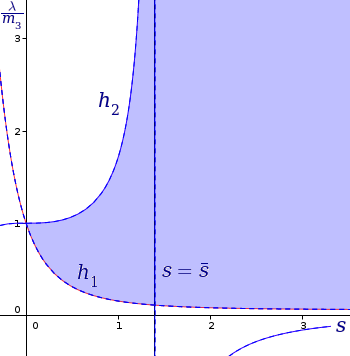
\includegraphics[width=2.7in, height=2.7in]{Lm3RegionSpecialCase.png}
 \caption{Region for $\frac{\lambda}{m_3}$ in terms of s. The blue region is the area where central configurations are possible.  }
\end{figure}
\end{center}


\section{Nonzero r Case Central Configuration}

\begin{theorem}
\label{thmsc}
\emph{Let $-1<r<1$, $r\neq0$, $s>0$, $t>0$, and $q=(-1-s,-1,r,1,1+t)$
with masses $m_{i}=f_{i}\lambda+f_{i}M$ respectively. Then it is possible for q to be a
central configuration if }
\begin{enumerate}
\item \emph{$0<r<1$ and $\frac{-f_{1}}{g_{1}}<\frac{M}{\lambda}<\frac{-f_{4}}{g_{4}}$.
For a given t, the possible configurations lie in the region under
the implicit curve $\frac{-f_{1}}{g_{1}}=\frac{-f_{4}}{g_{4}}$ in
regards to s and r.}
\item \emph{$-1<r<0$ and $\frac{-f_{5}}{g_{5}}<\frac{M}{\lambda}<\frac{-f_{2}}{g_{2}}$.
For a given t, the possible configurations lie in the region under
the implicit curve $\frac{-f_{5}}{g_{5}}=\frac{-f_{2}}{g_{2}}$ in
regards to t and r.}\end{enumerate}
\end{theorem}

In order to find determine the parameters for central configurations, we need to find where we have positive masses. For $i={1,2,...5} m_i = f_i\lambda + g_iM > 0$. In theorem 1.\ref{willthm}, it was shown that $g_1 > 0, g_3 > 0, g_5 > 0, g_2 < 0, g_4 < 0$. Using this, we can rewrite the inequalities thusly: 

\begin{equation} \begin{array}{ll}
m_1: & \frac{M}{\lambda} > \frac{-f_1}{g_1} \\
m_2: & \frac{M}{\lambda} < \frac{-f_2}{g_2} \\
m_3: & \frac{M}{\lambda} > \frac{-f_3}{g_3} \\
m_4: & \frac{M}{\lambda} < \frac{-f_4}{g_4} \\
m_5: & \frac{M}{\lambda} > \frac{-f_5}{g_5} \\
\end{array}
\end{equation}

Thus, central configurations are possible when $max(\frac{-f_1}{g_1},\frac{-f_3}{g_3},\frac{-f_5}{g_5})<\frac{M}{\lambda}<min(\frac{-f_2}{g_2},\frac{-f_4}{g_4})$. To simplify notation, we will refer to $-\frac{f_i}{g_i}$ as $min_i$ for $i={1,3,5}$ and $max_i$ for $i={2,4}$ Initially, we chose a value for r and plotted the region in terms of s and t. Then, we chose a value for t and plotted the region for s and r. When we picked a value for t and plotted the region in terms of s and r, we found that the region closely approximates a parabola. The regions appear to approach the parabola in the $t=1$ plane and then begin to decline.

\begin{center}

\begin{figure}
\label{rfix}
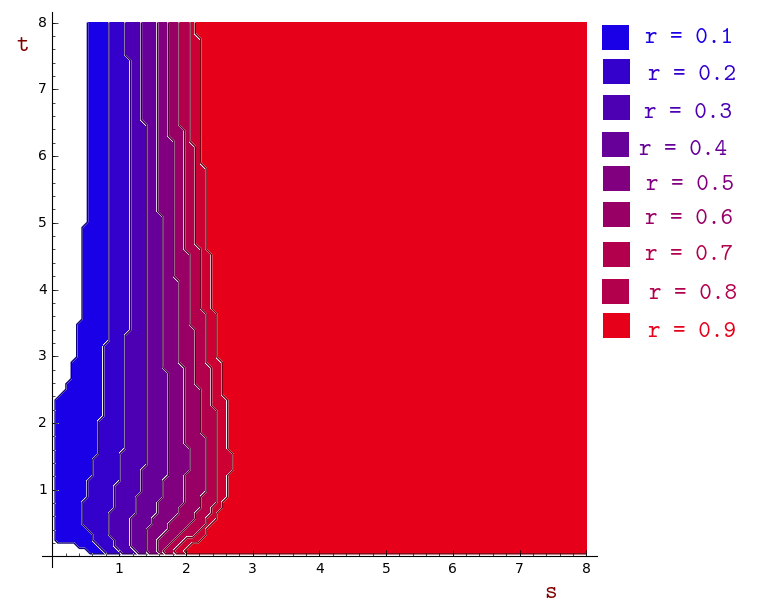
\includegraphics[width=3.9in, height=3in]{regionsRfixed.png}
 \caption{   Plots of the regions where central configurations are possible for given values of r in terms of s and t.} 
\end{figure}

\begin{figure}
\label{tfix}
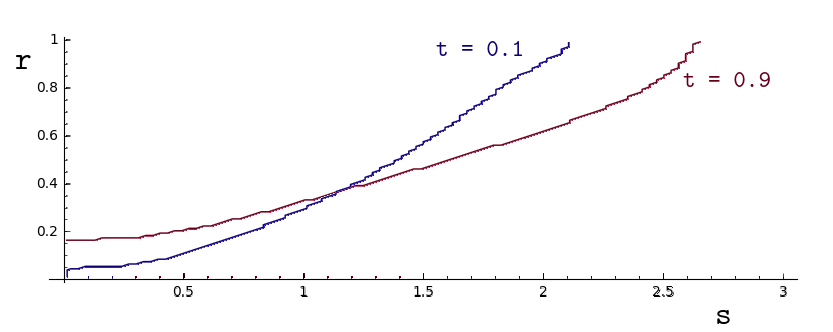
\includegraphics[width=6in, height=2in]{regionstLessThan1.png}
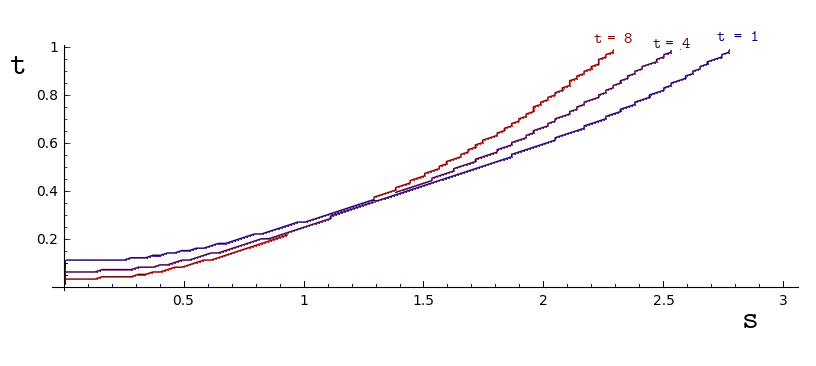
\includegraphics[width=6in, height=2in]{regionst18.png}
 \caption{   Plots of the regions where central configurations are possible for given values of t in terms of r and s. Central configurations are possible in the regions under the curves.} 
\end{figure}

\end{center}


Therefore, we explored the regions for $t = 1$ further. First, as shown in figure \ref{rg0o}, we plotted the implicit curves $min_1=min_3, min1=min_5,min_3=min_5$ to outline the regions for the minimum values and $\frac{-f_2}{g_2},\frac{-f_4}{g_4}$ to outline the regions for the maximum values. Then, we looked at the regions where $\frac{-f_1}{g_1}$ is greater than both $\frac{-f_3}{g_3}$ and $m_5$ and likewise for $\frac{-f_3}{g_3}$ and $m_5$ and where $-\frac{f_2}{g_2}>m_4$ and $m_4>\frac{-f_2}{g_2}$. Next, we superimposed the regions to see what our minimums and maximums would be for each region, which is shown in figure \ref{rg0r}. While we initially had five regions to consider, four regions turned out to be trivial cases where the maximum was always larger than the minimum over the entire region. The only region of interest is the $\frac{-f_1}{g_1} < \frac{-f_4}{g_4}$ region. Comparing the plot of $\frac{-f_1}{g_1} < \frac{-f_4}{g_4}$ (figure is a close to exact match for the previous plots of the the central configuration region in the $t=1$ plane. This is also the case when we choose different values for t as well.



\begin{center}

\begin{figure}
\label{rg0o}  
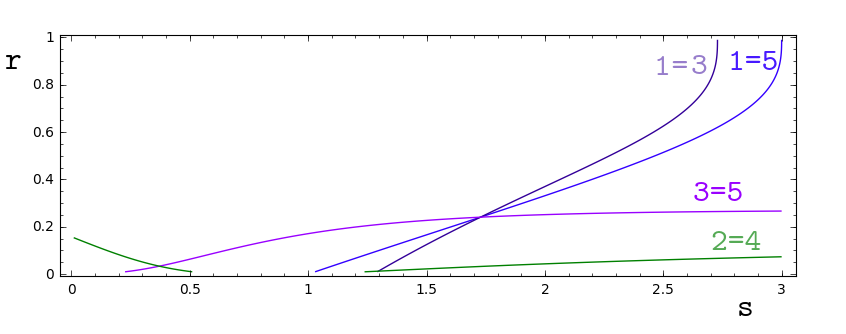
\includegraphics[width=6in, height=2in]{t1regionOutline.png}
 \caption{ Where $-\frac{f_i}{g_i}=-\frac{f_i}{g_i}$ for specified $i$ in the $t=1$ plane. Notation is simplified in the figure. For example, 1 represents $-\frac{f_1}{g_1}$.} 
\end{figure}

\begin{figure}
\label{rg0r} 
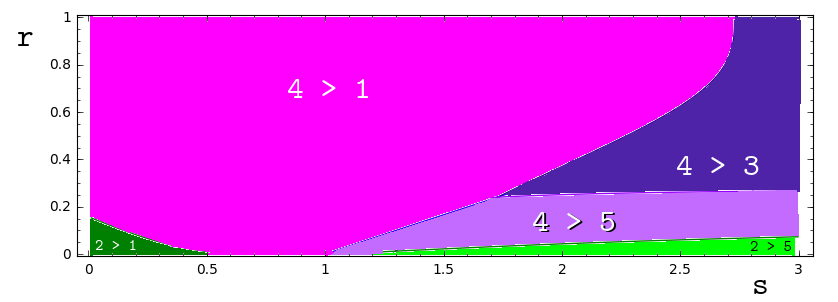
\includegraphics[width=6in, height=2in]{t1rG0region.png}
 \caption{  Conditions for central configuration for specified regions of $r$ and $s$ in the $t=1$ plane. Notation is simplified in the figure. For example, 1 represents $-\frac{f_1}{g_1}$.}
\end{figure}

\end{center}

We can then rotate the configuration to look at $r<0$. When $r<0$, the configuration is the same as the $r>0$ configuration, but t and s are swapped. Also, $m1$ becomes $m5$ and $m2$ becomes $m4$. Therefore, the defining curve for $r<0$ is $-\frac{f_5}g_5}=-\frac{f_2}{g_2}$ and $-\frac{f_5}{g_5}<\frac{M}{\lambda}<-\frac{f_2}{g_2}$ for a central configuration to exist. This can be confirmed by plotting the region for a given t.


\begin{figure}
\label{f1g1}
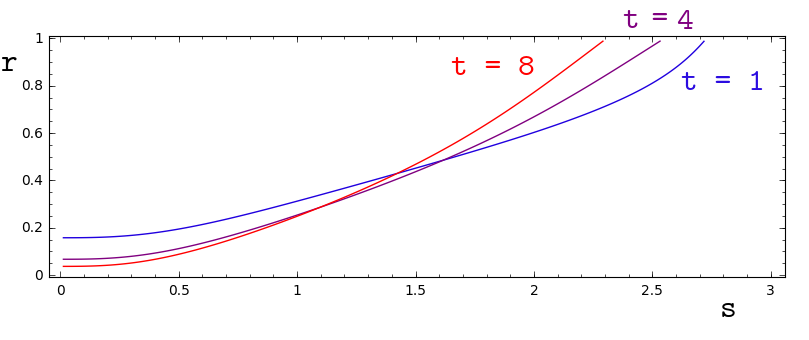
\includegraphics[width=6in, height=2in]{ict148.png}
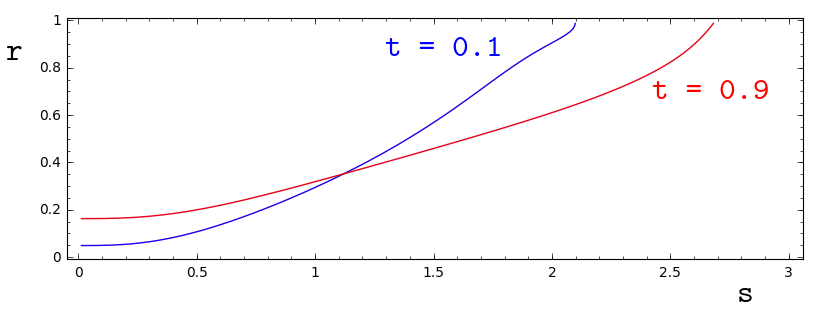
\includegraphics[width=6in, height=2in]{ictp1p9.png}
 \caption{   Plot of  $-\frac{f_1}{g_1} = -\frac{f_4}{g_4}$ for given values of t.}
\end{figure}

\end{center}

\section{r = 0 Case Central Configurations}

\begin{theorem}\label{scthm}
\emph{Let $s>0$, $t>0$, and $q=(-1-s,-1,0,1,1+t)$
with masses $m_{i}=f_{i}\lambda+f_{i}M$ respectively, then it is possible for q to be a
central configuration. }
\end{theorem}

Exploring the central configurations for the $r = 0$ case using the same method as the $r > 0$ case, we can seperate the problem into six regions based on the maximum of $m_1,m_2,m_3$ and the minimum of $m_2,m_4$. If we rotate the configuration, half of these cases are identical. This can also be observed in the symmetry of the figure. If we swap the s and t axises and $f_1,g_1$ and $f_5,g_5$ and $f_2,g_2$ and $f_4,g_4$, we would have an identical graph. Therefore, we can look at three of these regions to see if $-f_5/g_5 < -f_4/g_4$, $-f_5/g_5<-f_2/g_2$, and $-f_3/g_3<-f_4/g_4$. For each of these regions, the maximum value is always larger than the minimum value. 

\begin{figure}
\includegraphics[width=6in, height=6in]{rIsZeroRegions.png}
 \caption{ \label{EL}  Conditions for central configuration for specified regions of $r$ and $s$ in the $t=1$ plane. Notation is simplified in the figure. For example, 1 represents $-\frac{f_1}{g_1}$.}
\end{figure}


\section{Permutations for Super Central Configurations}
As the number of possible permutations of 5 masses is large, it would be better if we could eliminate some of the permutations prior to having to write them down. This can be done relatively easily and in a way that should extend to super central configurations of the collinear n-body problem. First we shall prove the following lemma in a similar manner to how it was proved in \cite{ZX3}. It is important to keep in mind that the mass distribution is entirely determined by $M, \lambda, r,s,$ and $t$; and when investigating the super central configurations, all are held fixed.

\begin{lemma}
\begin{enumerate}
Fix $q=(-s-1, -1, r, 1, t+1)$ with $(s,t)\in \mathbf{R^+}^3$ and $-1<r<1$. Suppose $m=(m_1, m_2, m_3, m_4, m_5)\in S(q)$ and $\tau \in P(5)$. 
\item If $m(\tau)\in S(q)$ and $m_{\tau(i)}=m_i$, then $m(\tau)=m$.
\item If $m(\tau) \in S(q)$, $m_{\tau(i)}=m_j$, and $m_{\tau(j)}=m_i$; then $m_i=m_j$.
\end{enumerate}
\end{lemma}

\textit{Proof of Lemma 4.1}
\begin{enumerate}
\item If $m_{\tau(i)}=m_i$ for some $i$, we can assume without loss of generality that $i=1$ which gives
$$ m_1=\lambda f_1+M g_1=\lambda_\tau f_1+M g_1=m_{\tau(1)}$$. This, shows that $\lambda_\tau=\lambda$. We know that the mass distribution is entirely fixed for a given $r,s,t,\lambda,$ and $M$ and so if $\lambda_\tau=\lambda$ then then $m(\tau)=m$.

\item If $m_{\tau(i)}=m_j$ and $m_{\tau(j)}=m_i$, then we have that $m_i=\lambda f_i +M g_i=\lambda_\tau f_j + M g_j=m_{\tau(j)}$ and $m_j=\lambda f_j +M g_j=\lambda_\tau f_i + M g_i=m_{\tau(i)}$. If $\lambda_\tau=\lambda$ then by a simple comparison of terms, we have $m_i=m_j$. Assume $\lambda_\tau \neq \lambda$. by adding $m_i$ and $m_j$ we get $m_i+m_j=m_{\tau(j)}+m_{\tau(i)}$, or 
$$\lambda f_i +M g_i+\lambda f_j +M g_j=\lambda_\tau f_j +M g_j+\lambda_\tau f_i + M g_i $$
$$\lambda (f_i +f_j) +M (g_i+g_j)=\lambda_\tau (f_i+f_j)+M(g_i+g_j)$$
Assuming $f_i+f_j \neq 0$, this gives $\lambda_\tau=\lambda$. This is a contradiction meaning our initial assumption that $\lambda_\tau \neq \lambda$ is false. By having $\lambda_\tau=\lambda$ we have that the mass distribution is entirely defined by $M, \lambda, r,s,t$ and have that $m=m(\tau)$
\end{enumerate}
Thus the Proof of Lemma 6.1 is complete.

By using this lemma, we are able to reduce the number of cases that must be checked by hand in order to find the super central configurations. To begin with there were $5!=120$ permutations that needed to be checked. 
However, part 1 of Lemma 6.1 allows us to remove all permutations that are not derangements; and part 2 of Lemma 6.1 allows us to remove from the list of derangements all permutations that have two masses swapping their respective locations. 
The number of derangements of n objects is typically written as $!n$ and $!5=44$. the second part of Lemma 6.1 allows us to remove an additional ${n \choose 2} (!(n-2))$ from the derangements. 
This leaves $!5-{5\choose 2}(!3)=24$ permutations that must be checked by hand. We will denote the permutation $(1,2,3,4,5)$ as $\tau$ and it shall not be counted among the $24$. We will have to discuss the following $24$ permutations of $5$ masses in order to find the possible super central configurations:

$$ \tau_1=(2,4,1,5,3),\hspace{1cm} \tau_2=(2,5,1,3,4),\hspace{1cm} \tau_3=(2,5,4,1,3),\hspace{1cm} \tau_4=(2,3,5,1,4)$$
$$ \tau_5=(2,3,4,5,1),\hspace{1cm} \tau_6=(2,4,5,3,1),\hspace{1cm} \tau_7=(3,1,4,5,2),\hspace{1cm} \tau_8=(3,1,5,2,4)$$
$$ \tau_9=(3,5,2,1,4),\hspace{1cm} \tau_{10}=(3,4,5,1,2),\hspace{1cm} \tau_{11}=(3,4,2,5,1),\hspace{1cm} \tau_{12}=(3,5,4,2,1)$$
$$ \tau_{13}=(4,1,5,3,2),\hspace{1cm} \tau_{14}=(4,1,2,5,3),\hspace{1cm} \tau_{15}=(4,5,1,2,3),\hspace{1cm} \tau_{16}=(4,3,1,5,2)$$
$$ \tau_{17}=(4,5,2,3,1),\hspace{1cm} \tau_{18}=(4,3,5,2,1),\hspace{1cm} \tau_{19}=(5,1,2,3,4),\hspace{1cm} \tau_{20}=(5,1,4,2,3)$$
$$ \tau_{21}=(5,3,1,2,4),\hspace{1cm} \tau_{22}=(5,4,1,3,2),\hspace{1cm} \tau_{23}=(5,4,2,1,3),\hspace{1cm} \tau_{24}=(5,3,4,1,2)$$

\section{Special Cases for Super Central Configurations}

Before trying to make any statements about the general super central configurations, it would be beneficial to first investigate the cases where we have some equal masses. 
It is known that it is impossible to have $3$ or $4$ equivalent masses because both cases would violate Lemma 4.1. This leaves the case where we have $2$ equivalent masses and $3$ distinct masses; as well as the case where we have two sets of $2$ equivalent masses with only one distinct mass. 

\begin{lemma}
Fix $q=(-s-1, -1, r, 1, t+1)$ with $(s,t)\in \mathbf{R^+}^3$ and $-1<r<1$. Suppose $m=(m_1, m_2, m_3, m_4, m_5)\in S(q)$ and $\tau \in P(5)$ Furthermore, assume that $m_i=m_j$ and $m_k=m_l$ with $i\neq j\neq k\neq l$ and $1\leq i,j,k,l \leq 5$. Then we shall have $m(\tau)\notin S_m(q)$ for all $\tau$.
\end{lemma}

\textit{Proof of Lemma 7.1}
First we shall define $a$ to be the number between 1 and 5 that is not $i,j,k,$ or $l$. We shall then assume that $\tau(a)\neq a$ because we know that that will not allow a super central configuration. Next, we shall assume without loss of generality that $\tau(i)=a$. From here there are two cases to examine. First we have the case $\tau(j)=i$ or $\tau(j)=j$; then there is also the case that $\tau(j)=k$ or $\tau(j)=l$. We will look at the first case first. 

We know from lemma 6.1 that $\tau(j)=j$ will not allow for a super central configuration so it is easily removed leaving only $\tau(j)=i$. In this case we will have $m_i=m_j=m_a$ because when $m_i=m_j$ then we must also have that the two masses taking their places in the configuration are equivalent. Thus with three equivalent masses we know that $\tau(j)=i$ will not all for a super central configuration.

This leaves only two more cases. By setting, $\tau(j)=k$, we get $m_a=m_k=m_l$ which gives us three equivalent masses. Finally, by assuming that $\tau(j)=l$, we get $m_a=m_k=m_l=m_{\tau(l)}$ and so we have $4$ equivalent masses. This completes the proof of Lemma 7.1.

\begin{lemma}
Fix $q=(-s-1, -1, r, 1, t+1)$ with $(s,t)\in \mathbf{R^+}^3$ and $-1<r<1$. Suppose $m=(m_1, m_2, m_3, m_4, m_5)\in S(q)$ and $\tau \in P(5)$ Furthermore, assume that $m_i=m_j$ with $i\neq j$ and $1\leq i,j \leq 5$. Then we shall have that $m(\tau) \notin S_m(q)$ for all $\tau$ if $f_i \neq f_j$.
\end{lemma}

\textit{Proof of Lemma 7.2:}
If $m_i=m_j$ then we have $\lambda f_i +Mg_i=\lambda f_j+Mg_j$. Additionally, because the two masses in the $i^{th}$ and $j^{th}$ positions must still be equal, we also have $\lambda_{\tau} f_i +Mg_i=\lambda_{\tau} f_j+Mg_j$. By subtracting the second equation from the first we get $(\lambda-\lambda_{\tau})f_i=(\lambda-\lambda_{\tau})f_j$.This is only true in two cases. Either $f_i=f_j$ and more analysis is required to see if a super central configuration exists, or $\lambda=\lambda_{\tau}$ and there is no super central configuration as shown in the previous section. This completes the proof of Lemma 7.2.




\section{General Case for Super Central Configurations}
We have from the first section the following equations:
$$m_1=f_1\lambda+Mg_1, \hspace{20pt} m_2=f_2\lambda+Mg_2, \hspace{20pt} m_3=f_3\lambda+Mg_3,$$
$$m_4=f_4\lambda+Mg_4, \hspace{20pt} m_5=f_5\lambda+Mg_5,$$
Then we also have the following equations when using the definition of super central configurations.
$$m_{\tau(1)}=f_1\lambda_\tau+Mg_1, \hspace{20pt} m_{\tau(2)}=f_2\lambda_\tau+Mg_2, \hspace{20pt} m_{\tau(3)}=f_3\lambda_\tau+Mg_3,$$
$$m_{\tau(4)}=f_4\lambda_\tau+Mg_4, \hspace{20pt} m_{\tau(5)}=f_5\lambda_\tau+Mg_5,$$
A useful result from the definition for the functions $f_i$ and $g_i$ is as follows.
\begin{lemma}
For any $-1<r<1$ and $s,t>0$
\begin{enumerate}
\item $f_1+f_2+f_3+f_4+f_5=0$
\item $g_1+g_2+g_3+g_4+g_5=1$
\end{enumerate}
\end{lemma}
\textit{Proof of Lemma 8.1}
We know that $m_1+m_2+m_3+m_4+m_5=M$ because that is how the total mass is defined. By substituting in the expressions for $m_i$ we get $(f_1+f_2+f_3+f_4+f_5)\lambda+(g_1+g_2+g_3+g_4+g_5)M=M$ as well as $(f_1+f_2+f_3+f_4+f_5)\lambda_\tau+(g_1+g_2+g_3+g_4+g_5)M=M$. 
Because a change in $\lambda$ does not cause a change in the total mass we must have $f_1+f_2+f_3+f_4+f_5=0$, which then clearly means $g_1+g_2+g_3+g_4+g_5=1$. And thus Lemma 8.1 is proved.


\textbf{Case 1:} $\tau_1=(2,4,1,5,3)$
Step 1: First we set $m_1=m_{\tau_1(3)}$ and $m_2=m_{\tau_1(1)}$. Then we solve for $\lamda$ and $\lambda_\tau_1$ by using the equations from above. This gives the following results:
$$\lambda=\frac{f_1g_3-f_1g_1+f_3g_2-f_3g_1}{{f_1}^2-f_2f_3}$$
$$\lambda_{\tau_1}=\frac{f_2g_3-f_2g_1+f_1g_2-f_1g_1}{{f_1}^2-f_2f_3}$$

Step 2: Substituting these $\lambda$ and $\lambda_\tau$ back into the original equations, then we get:
$$m_1=M\frac{{f_1}^2g_3-{f_1}^2g_1+f_1f_3g_2-f_1f_3g_1+{f_1}^2g_1-f_2f_3g_1}{{f_1}^2-f_2f_3}$$
$$m_2=M\frac{f_1f_2g_3-f_1f_2g_1+f_2f_3g_2-f_2f_3g_1+{f_1}^2g_2-f_2f_3g_2}{{f_1}^2-f_2f_3}$$
$$m_3=M\frac{f_1f_3g_3-f_1f_3g_1+{f_3}^2g_2-{f_3}^2g_1+{f_1}^2g_3-f_2f_3g_3}{{f_1}^2-f_2f_3}$$
$$m_4=M\frac{f_1f_4g_3-f_1f_4g_1+f_3f_4g_2-f_3f_4g_1+{f_1}^2g_4-f_2f_3g_4}{{f_1}^2-f_2f_3}$$
$$m_5=M\frac{f_1f_5g_3-f_1f_5g_1+f_3f_5g_2-f_3f_5g_1+{f_1}^2g_5-f_2f_3g_5}{{f_1}^2-f_2f_3}$$
as well as the following equations:
$$m_{\tau_1(1)}=M\frac{f_1f_2g_3-f_1f_2g_1+{f_1}^2g_2-f_2f_3g_1}{{f_1}^2-f_2f_3}$$
$$m_{\tau_1(2)}=M\frac{{f_2}^2g_3-{f_2}^2g_1+f_1f_2g_2-f_1f_2g_1+{f_1}^2g_2-f_2f_3g_2}{{f_1}^2-f_2f_3}$$
$$m_{\tau_1(3)}=M\frac{-f_2f_3g_1+f_1f_3g_2-f_1f_3g_1+{f_1}^2g_3}{{f_1}^2-f_2f_3}$$
$$m_{\tau_1(4)}=M\frac{f_2f_4g_3-f_2f_4g_1+f_1f_4g_2-f_1f_4g_1+{f_1}^2g_4-f_2f_3g_4}{{f_1}^2-f_2f_3}$$
$$m_{\tau_1(5)}=M\frac{f_2f_5g_3-f_2f_5g_3+f_1f_5g_2-f_1f_5g_1+{f_1}^2g_5-f_2f_3g_5}{{f_1}^2-f_2f_3}$$

Because these equations were created by assuming that $m_1=m_{\tau_1(3)}$ and $m_2=m_{\tau_1(1)}$, we must now investigate when it is possible to have $m_3=m_{\tau_1(5)}$, $m_4=m_{\tau_1(2)}$ and $m_5=m_{\tau_1(4)}$. This gives us the following three equations:
$$m_3-m_{\tau_1(5)}=M\frac{({f_1}^2-f_2f_3)(g_3-g_5)+(f_1f_3-f_2f_5)(g_3-g_1)+({f_3}^2-f_1f_5)(g_2-g_1)}{{f_1}^2-f_2f_3}=\frac{h_{11}M}{{f_1}^2-f_2f_3}$$
$$m_4-m_{\tau_1(2)}=M\frac{({f_1}^2-f_2f_3)(g_4-g_2)+(f_1f_4-{f_2}^2)(g_3-g_1)+(f_3f_4-f_1f_2)(g_2-g_1)}{{f_1}^2-f_2f_3}=\frac{h_{12}M}{{f_1}^2-f_2f_3}$$
$$m_5-m_{\tau_1(4)}=M\frac{({f_1}^2-f_2f_3)(g_5-g_4)+(f_1f_5-f_2f_4)(g_3-g_1)+(f_3f_5-f_1f_4)(g_2-g_1)}{{f_1}^2-f_2f_3}=\frac{h_{13}M}{{f_1}^2-f_2f_3}$$

We have from direct computation and using the fact that $f_1+f_2+f_3+f_4+f_5=0$ that $h_{11}+h_{12}+h_{13}=0$ for all $s,t > 0$ and $-1<r<1$. In order for $\tau_1$ to give a super central configuration we must have $h_{11}=0$, $h_{12}=0$, and $h_{13}=0$ all at the same time. However, because $h_{11}+h_{12}+h_{13}=0$, it is sufficient to have only $h_{11}=0$ and $h_{12}=0$.

\textbf{Case 2:} $\tau_2=(2,5,1,3,4)$


\section*{Acknowledgment}

%The author would like to thank Dr. Chi-Kwong Li for some valuable discussion on the properties of Pfaffian, especially the simple proof of theorem \ref{Pf6}.

\begin{thebibliography}{00}

\bibitem{AM} A. Albouy and R. Moeckel, The inverse problem
for collinear central configuration, Celestial Mechanics and
Dynamical Astronomy 77 (2000), 77--91.

\bibitem{AC} Arthur Cayley, On the theory of permutants, Cambridge and Dublin Mathematical Journal VII:
(1852) 40�51 Reprinted in Collected mathematical papers, volume 2.


\bibitem{Buch} H.E. Buchanan, On certain determinants connected with a problem in Celestial Mechanics, Bull. Amer. Math. Soc. 5 (1909), 227-231.

\bibitem{EL} L. Euler, De motu rectilineo trium corporum se mutuo attahentium, Novi Comm. Acad. Sci. Imp. Petrop. 11 (1767), 144-151.

\bibitem{LA} J. Lagrange,Essai sur le probl\`{e}me des trois corps. Euvres, vol. 6, Gauthier-
Villars, Paris, 1772, pp. 272�292 % Collected works, Vol 6 (1772), 229-324.

\bibitem{LS} Y. Long and S.  Sun, Collinear Central
Configurations and Singular Surfaces in the Mass Space, Arch.
Rational Mech. Anal. 173 (2004) 151-167.
\bibitem{LS2} Y. Long and S.  Sun, "Collinear central
configurations in celestial mechanics", Topological Methods,
Variational Methods and Their Applications: ICM 2002 Satellite
Conference on Nonlinear Functional Analysis, Taiyuan, Shan Xi, P.R.
China, August 14 - 18, 2002 By H. Brezis, K. C. Chang, p159--165.

\bibitem{MN} F.R. Moulton, The straight line solutions of the
problem of $N$-bodies, Ann. Math. 2(12)(1910), 1-17 (or in his book:
Periodic Orbits, published by the Carnegie Institution of
Washington, 1920, 28-298).

\bibitem{OX1} T. Ouyang, Z. Xie, Collinear Central Configuration in Four-body Problem,
 Celestial Mechanics and Dynamical Astronomy, Vol. 93(2005),
 147-166.

 \bibitem{ZX4} T. Ouyang, Z. Xie, Number of Central Configurations and Singular Surfaces in
Mass Space
in the Collinear Four-body Problem. Transactions of the American Mathematical Society,364 (2012), 2909-2932.

\bibitem{Win} A. Wintner, The Analytical Foundations of Celestial Mechanics. Princeton
Math. Series 5, 215. Princeton Univ. Press, Princeton, NJ. 1941. 3rd
printing 1952.

 \bibitem{ZX2} Z. Xie, Super Central Configurations of the $n$-body Problem.
 Jour. Math. Physics, 51, (2010) 042902.


\bibitem{ZX3} Z. Xie, Inverse Problem of Central Configurations and Singular Curve in the Collinear $4$-Body
  Problem,  Celestial Mechanics and Dynamical
Astronomy 107, (2010) 353�-376.

\bibitem{ZX5} Z. Xie, Central Configurations of the Collinear Three-body Problem and Singular Surfaces in the Mass Space. Physics Letters A, 375 (2011) 3392�-3398.
\bibitem{ZX6} Z. Xie, An analytical proof on certain determinants connected with the collinear central configurations in the $n$-body problem, Celestial Mechanics and Dynamical
Astronomy 118 (2014), no. 1, 89-97.
\end{thebibliography}
\end{document} 

